\documentclass[11pt]{article}
\usepackage[T1]{fontenc}
\usepackage{lmodern,microtype,amsmath,amssymb,amsthm,mathtools}
\usepackage[margin=1in]{geometry}
\usepackage{graphicx,booktabs,array,longtable,xcolor,enumitem}
\usepackage[colorlinks=true,linkcolor=blue!45!black,urlcolor=blue!55!black,citecolor=blue!45!black]{hyperref}
\hypersetup{pdftitle={When the control record arrives: a finite-error memory law for one quantum payload},pdfauthor={Constructed research return},pdfsubject={Causal quantum acquisition and quantum memory bounds}}
\setlength{\parskip}{3pt}
\setlength{\parindent}{0pt}
\setlist{nosep,leftmargin=*}
\newtheorem{theorem}{Theorem}
\newtheorem{lemma}[theorem]{Lemma}
\newtheorem{corollary}[theorem]{Corollary}
\newcommand{\Tr}{\operatorname{Tr}}
\newcommand{\id}{\operatorname{id}}
\newcommand{\supp}{\operatorname{supp}}
\newcommand{\Ad}{\operatorname{Ad}}
\newcommand{\dd}{d_{\diamond}}
\newcommand{\norm}[1]{\left\lVert#1\right\rVert}
\title{When the control record arrives:\\a finite-error memory law for one quantum payload}
\author{Constructed research return with independent audits}
\date{5 November 2026}
\begin{document}
\maketitle
\begin{abstract}
A stream may contain only one arbitrary qubit of recoverable payload yet
require extensive quantum memory before a short classical control record
arrives. We give a quantitative theorem for this task, allowing unlimited
classical records, arbitrary receiver processing and a different final decoder
for every record. If balanced encoding observables have commutator gap
$\kappa$, a receiver with quantum dimension at most $m$ in each classical
branch and selector-averaged half-diamond error $\epsilon\le1/2$ must satisfy
$m\ge N[1-8\epsilon(1-\epsilon)/\kappa]$, where $N$ is the early register's
dimension. A common Petz reconstruction is constructed only as a proof
witness; whole-output reconstruction is not required of the receiver.

A small-bias Pauli construction gives $\kappa\ge4/5$, a once-through tracial
stream of $n$ carriers and one late payload flag, a $2\lceil\log_2(4n-2)\rceil+1$
bit record, and one coherent source qubit. Delivering that record before the
carriers permits exact arbitrary-reference recovery by local measurements,
one classical parity and a final one-qubit correction: linear quantum work,
constant coherent receiver workspace and near-linear classical work. At one
percent error, delaying the same record requires $m\ge0.901\,2^{n+1}$, so a
receiver must provision all $n+1$ whole qubits of capacity at the critical cut;
individual classical branches may retain fewer. A separate imported local expander gives a five-bit record and
constant total logical source dimension, with a much smaller certified error
threshold. These are complete programmed-source constructions, not a decoder
for the homogeneous weak partial-SWAP stream. Strong encounters, paid source
coherence, the actual timing of the control record and implementation accuracy
are part of the statements.
\end{abstract}

\section{The selected question and its consequence}

The completed fourth-order action law determines how much mixed-particle
interaction is necessary for physical output acquisition. It does not determine
how much quantum memory a receiver must keep. The next question selected here is:
\begin{quote}
Can the dimension of a small recoverable payload, or of a small emitting source,
bound the quantum memory of a causal receiver when its physical inputs are mixed?
Which additional classical access makes a small receiver possible?
\end{quote}
The answer is a quantitative obstruction with a matching positive interface.
The relevant distinction is the arrival time of a record specifying the source's
encoding. A short early record can enable immediate local measurements and exact
recovery. The same record delivered later can force retention of essentially all
quantum carriers, even though the final requested output is one qubit.

The mathematical novelty claimed in this return is limited to the derivation
and composition given here. Late-choice quantum-memory phenomena are established
\cite{bww,brw}; environmental measurement and correction are established
\cite{gw}; small-bias Pauli randomization is established \cite{aghp,as}.
We supply an explicit finite-error bridge under the weaker, payload-specific
recovery premise and complete physical stream constructions. No historical
priority, laboratory demonstration, or realised civilisation-scale benefit is
asserted. The result does rule out a general compact mixed-stream receiver based
only on payload dimension, and identifies an access resource that removes the
obstruction in the constructed family.

Independent selection initially pursued the weak partial-SWAP receiver, thermal
identification from partial observation, raw-image hydrodynamic force acquisition,
and this foundational memory question. The latter yielded the strongest closed
theorem and operation. The other completed results are retained as companions,
with their actual costs and boundaries in Section~\ref{sec:companions}.

\section{Operational contract}

The payload $Q$ is an arbitrary qubit, possibly entangled with an arbitrary
reference $R$. A classical selector $j$, independent of $QR$, specifies a known
encoding. The early quantum register $B$ has dimension $N=2D$ and is
\begin{equation}
 \mathcal E_j(\rho)=V_j(\rho\otimes I_D/D)V_j^\dagger. \label{eq:encode}
\end{equation}
All of $B$ arrives before $j$ in the hard interface. The receiver applies one
common channel $\mathcal C$ before seeing $j$. Its retained state consists of an
arbitrary classical record and a quantum register of dimension at most $m$ in
every classical branch. After learning $j$, it may use any channel $\mathcal D_j$
to return one qubit. Fresh decoder ancillas are allowed. There is no uncounted
quantum memory, entanglement half, output delay line or coherent external record
across the cut. No initial entanglement with the source is supplied.

We use the half-diamond convention throughout:
\begin{equation}
 \dd(\mathcal A,\mathcal B)=\tfrac12\norm{\mathcal A-\mathcal B}_{\diamond}.
\end{equation}
The sufficient performance premise is only
\begin{equation}
 \dd\left(\sum_jp_j\mathcal D_j\mathcal C\mathcal E_j,\id_Q\right)
 \le\epsilon. \label{eq:performance}
\end{equation}
A worst-selector or flagged reference-uniform guarantee implies this premise.
The different $\mathcal D_j$ need not reconstruct the full state of $B$, preserve
every mixed-output correlation, or be related to one another.

The bound is on quantum dimension in every classical branch, not expected
qubit count. It allows arbitrary adaptive measurements and classical feedback
inside the receiver. In fact it allows a collective operation on all of $B$
before the cut, and therefore also bounds every causal once-through receiver.
The source follows its declared program; receiver feedback cannot reprogram it
to release the payload or selector earlier. Failure/postselection is not omitted
from \eqref{eq:performance}.

\section{The memory theorem}

Let $H_j=V_j(Z\otimes I_D)V_j^\dagger$. These are traceless Hermitian
involutions. Assume the following quantitative irreducibility for every complex
$N\times N$ matrix $K$, using unnormalised Hilbert--Schmidt norms:
\begin{equation}
 \sum_jp_j\norm{[K,H_j]}_2^2\ge
 \kappa\norm{K-\tfrac{\Tr K}{N}I_N}_2^2. \label{eq:gap}
\end{equation}

\begin{theorem}[Payload memory with a late selector]\label{thm:memory}
Under \eqref{eq:encode}--\eqref{eq:gap}, for $0\le\epsilon\le1/2$,
\begin{equation}
 \boxed{\frac mN\ge 1-\frac{8\epsilon(1-\epsilon)}{\kappa}.} \label{eq:main}
\end{equation}
The lower bound can be replaced by zero when negative. In particular,
$\epsilon\le\kappa/16$ implies $m\ge N/2$. Exact recovery requires $m\ge N$.
\end{theorem}

\begin{proof}
Set $\sigma=\mathcal C(I_N/N)$ and $x_j=\mathcal C(H_j)/N$.
Positivity gives $-\sigma\le x_j\le\sigma$, so
$t_j=\norm{x_j}_1\in[0,1]$. The two payload inputs $|0\rangle,|1\rangle$
encode as $(I_N\pm H_j)/N$. Their optimum discrimination bias after
compression is $t_j$. Measuring $Z$ after $\mathcal D_j$ is an allowed,
possibly suboptimal test. Applying \eqref{eq:performance} to each of these
two inputs shows that its selector-averaged success probability is at least
$1-\epsilon$. Consequently
\begin{equation}
 \sum_jp_jt_j\ge1-2\epsilon. \label{eq:bias}
\end{equation}

Construct the Petz map relative to the full-rank input $I_N/N$:
\begin{equation}
 \mathcal R(X)=\frac1N\mathcal C^*\bigl(\sigma^{-1/2}X\sigma^{-1/2}\bigr).
 \label{eq:petz}
\end{equation}
Inverses are on $\supp\sigma$. Every output of $\mathcal C$ is supported
there. The map is completely positive and trace preserving on that support,
since $\mathcal C(I_N)=N\sigma$; extend it arbitrarily to a trace-preserving
map on the unused complement. Thus $\mathcal T=\mathcal R\mathcal C$ is a
channel through the same hybrid memory. Define
\begin{equation}
 q_j=\frac1N\Tr[H_j\mathcal T(H_j)]
 =\Tr[x_j\sigma^{-1/2}x_j\sigma^{-1/2}].
\end{equation}
For $A_j=\operatorname{sign}(x_j)$, extended as a Hermitian contraction,
weighted Cauchy--Schwarz yields
\begin{align}
 t_j^2
 &\le \Tr[\sigma^{1/2}A_j\sigma^{1/2}A_j]\,q_j\le q_j. \label{eq:bridge}
\end{align}
For completeness, the first factor is
$\sum_{ab}\sqrt{\sigma_a\sigma_b}|(A_j)_{ab}|^2$ in an eigenbasis of
$\sigma$. Using $\sqrt{uv}\le(u+v)/2$ and $A_j^2\le I$ bounds it by
$\Tr\sigma=1$.

Write $\mathcal T(X)=\sum_\ell K_\ell X K_\ell^\dagger$. Trace preservation
and $H_j^2=I$ give the exact identity
\begin{equation}
 \sum_\ell\norm{[K_\ell,H_j]}_2^2
 =2N-2\operatorname{Re}\Tr[H_j\mathcal T(H_j)].
\end{equation}
Applying \eqref{eq:gap} to each Kraus operator gives
\begin{align}
 F_e(\mathcal T)
 &=N^{-2}\sum_\ell|\Tr K_\ell|^2\\
 &\ge1-\frac2\kappa\left(1-\sum_jp_jq_j\right)\\
 &\ge1-\frac2\kappa\left[1-\left(\sum_jp_jt_j\right)^2\right]
 \ge1-\frac{8\epsilon(1-\epsilon)}\kappa. \label{eq:fe}
\end{align}
Here Jensen's inequality and \eqref{eq:bridge} supply the middle step.

Every composite Kraus operator of a channel through dimension $m$ in each
classical branch has rank at most $m$. Therefore
$|\Tr K_\ell|^2\le m\Tr K_\ell^\dagger K_\ell$, and
$F_e(\mathcal T)\le m/N$. Equivalently its Choi state has Schmidt number at
most $m$, whose overlap with an $N$-dimensional Bell state is at most $m/N$.
This argument is independent of the classical alphabet size; its closed-convex
form also covers limits of dephased classical records. Combining with
\eqref{eq:fe} proves the theorem.
\end{proof}

The key step is \eqref{eq:bridge}. The actual task allows a different decoder
after every selector and returns only a qubit. It does not supply a common
whole-output reconstruction. The proof manufactures one analytically from
the compression channel. No efficient physical implementation of
\eqref{eq:petz} is assumed or needed.

\subsection{Causal prefixes and retained quantum exposure}\label{sec:prefix}
Suppose $B$ consists of $s$ qubits emitted in a fixed order, with the selector
only afterward. Let $\mathcal C_\ell$ be the receiver's operation after the
first $\ell$ qubits. Because future source operations do not act on emitted
qubits or depend on receiver feedback, $\mathcal C_\ell$ can be deferred
algebraically to act on the corresponding prefix of the complete emitted state.
Granting the receiver the untouched suffix for free gives a valid compression
$\mathcal C_\ell\otimes\id_{\rm suffix}$ through dimension at most
$m_\ell2^{s-\ell}$ per classical branch. Theorem~\ref{thm:memory} implies
\begin{equation}
 \frac{m_\ell}{2^\ell}\ge r_\epsilon,
 \qquad r_\epsilon=1-\frac{8\epsilon(1-\epsilon)}\kappa. \label{eq:prefix}
\end{equation}
Thus the obstruction occurs throughout the stream, not only at its end.
For $r_\epsilon>1/2$, a provisioned register of whole qubits needs capacity
at least $\ell$ after every prefix.

Variable branch sizes can also be charged without adding maxima from
incompatible histories. Let branch $y$ retain $q_y=\log_2m_y$ qubits of
dimension. Under the maximally mixed payload (or the marginal of a Bell input),
the prefix baseline is $I/2^\ell$. The branchwise rank proof for the Petz
witness gives
\begin{equation}
 r_\epsilon\le F_e(\mathcal T)
 \le\mathbb E\,2^{\min(q_y,\ell)-\ell}.
\end{equation}
Indeed each branch of the Petz reconstruction is trace preserving on that
branch's support, so its Kraus squared norms sum to the baseline branch
probability times the input dimension. The prefix input additionally bounds
each compression Kraus rank by $2^\ell$. Convexity places $2^{x-\ell}$ below
the chord connecting $x=0$ and $x=\ell$, yielding
\begin{equation}
 \mathbb E q_y\ge
 \max\left\{0,\frac{\ell(r_\epsilon-2^{-\ell})}{1-2^{-\ell}}\right\}.
 \label{eq:meanmemory}
\end{equation}
This expectation is for the stated baseline input; it supplies a worst-input
resource lower bound for a reader required to work on arbitrary inputs.

If arrivals are separated by at least $\tau$, apply the same argument at
every time between arrivals and integrate. The expected retained qubit-time
before the selector is at least
\begin{equation}
 \tau\sum_{\ell=1}^{s-1}
 \max\left\{0,\frac{\ell(r_\epsilon-2^{-\ell})}{1-2^{-\ell}}\right\}.
 \label{eq:exposure}
\end{equation}
For fixed positive $r_\epsilon$ this is $\Omega(\tau s^2)$. At one percent
in the small-bias construction, $r_\epsilon=0.901$. This is an actual
mean-exposure lower bound, not a sum of branchwise worst-case costs. Extra
waiting before any selector information arrives obeys the same prefix bound.
Progressive header disclosure requires a conditional-ensemble analysis.
Source feedback that changes the
encoding would invalidate the deferred-prefix step and is an extra interface.

\subsection{An experimentally scored consequence}

Choose $j$ with probability $p_j$ and an independent uniform sign. Prepare
$(I_N\pm H_j)/N$, hide the labels during compression, then disclose only $j$
and ask for the sign. If the average error is $q\le1/2$, the same proof gives
\begin{equation}
 \frac mN\ge1-\frac{8q(1-q)}\kappa
 =1-\frac2\kappa(1-s^2),\qquad s=1-2q. \label{eq:witness}
\end{equation}
This witnesses quantum memory under trusted preparation; a high score alone
does not establish arbitrary-payload recovery. For $M$ independent trials of
a fixed device with signed mean $\widehat s$ and trusted score bias at most
$\nu$, Hoeffding gives
\begin{equation}
 s_{\rm low}=\max\{0,\widehat s-\sqrt{2\log(1/\delta)/M}-\nu\}
\end{equation}
with confidence $1-\delta$. Substitution in \eqref{eq:witness} gives a finite
certificate. The per-trial physical preparation still uses $n$ carriers and
$O(n)$ operations. The claim is not device independent, does not exclude
unmodelled quantum side channels, and does not count only successful trials.

If all $M$ signed trials succeed and trusted bias is zero, the exact binomial
bound is $q\le1-\delta^{1/M}\le\log(1/\delta)/M$. Therefore
$M\ge8\log(1/\delta)/(\kappa\eta)$ suffices to certify $m/N\ge1-\eta$.
For the small-bias gap $\kappa=4/5$, $\eta=0.1$ and confidence $95\%$, 300
zero-failure trials suffice. This is a calculated ideal qualification point,
not an executed 1000-qubit experiment. Nonzero trusted bias must be subtracted.
Each trial uses one known pure payload qubit, $n$ tracial carriers, the paid
source control and delayed record, and one final bit. Applying the prefix
argument to the same score also certifies the mean retained quantum exposure
in \eqref{eq:exposure}; the test does not certify universal recovery merely
because it certifies that the receiver had to preserve quantum memory.

\section{A short explicit control record with a useful gap}

\subsection{A balanced Hermitian lift}
Suppose Hermitian involutions $U_j$ on a $D$-dimensional gauge register have
average conjugation $\Phi$ with absolute Hilbert--Schmidt contraction at most
$1-\gamma$ on traceless matrices. Use
\begin{equation}
 H_0=Z\otimes I_D,\quad H_j=X\otimes U_j,\quad
 p_0=\alpha,\quad \sum_{j\ne0}p_j=1-\alpha. \label{eq:lift}
\end{equation}
The conditional distribution on $j\ne0$ is that of $\Phi$. Then
\begin{equation}
 \kappa\ge\min\{4\alpha,\;2(1-\alpha)\gamma\}. \label{eq:liftgap}
\end{equation}
To see this, decompose $K=I\otimes A+X\otimes B+Y\otimes C+Z\otimes E$.
Average conjugation by \eqref{eq:lift} is block diagonal in these four flag
sectors. On the gauge-traceless part, the largest possible eigenvalue is at
most $1-(1-\alpha)\gamma$. The remaining nonscalar flag modes have gaps
$2\alpha$, $2$ and $2(1-\alpha)$ from eigenvalue one. Commutator energy is
twice this spectral deficit, proving \eqref{eq:liftgap} for complex $K$.
The $Z$ anchor is essential: $X\otimes I_D$ commutes with every $X\otimes U_j$.

The encoders are
\begin{equation}
 V_0=I,\qquad V_j=\left(|0\rangle\langle0|\otimes U_j+
 |1\rangle\langle1|\otimes I_D\right)(H\otimes I_D). \label{eq:controlled}
\end{equation}
Here $H$ is Hadamard. Direct multiplication gives
$V_j(Z\otimes I_D)V_j^\dagger=X\otimes U_j$.

\subsection{Small-bias Pauli construction}
The following finite-field construction is standard small-bias machinery
\cite{aghp}; the Pauli connection is established \cite{as}. We include the
calculation so the gap does not depend on an unspecified random family.

Let $r=2n$, $k=\lceil\log_2(2(r-1))\rceil$, $q=2^k$, and choose $a,b$
uniformly in $\mathbb F_q$. For $0\le\ell<r$, set
\begin{equation}
 x_\ell=\operatorname{tr}_{\mathbb F_q/\mathbb F_2}(ab^\ell),\qquad b^0=1.
\end{equation}
For every nonzero $v\in\mathbb F_2^r$, let
$f_v(z)=\sum_{\ell=0}^{r-1}v_\ell z^\ell$. Uniformity of $a$ gives
\begin{equation}
 \mathbb E_{a,b}(-1)^{v\cdot x}
 =\Pr_b\{f_v(b)=0\}\le\frac{r-1}{q}\le\frac12. \label{eq:biasfield}
\end{equation}
The equality uses nondegeneracy of the field trace; the inequality counts
roots of a nonzero polynomial. The biases are also nonnegative.

Pair the bits into $n$ Hermitian one-qubit Paulis,
\begin{equation}
 P_{a,b}=\bigotimes_{i=0}^{n-1}
 i^{x_{2i}x_{2i+1}}X^{x_{2i}}Z^{x_{2i+1}}.
\end{equation}
Every nonidentity Pauli is an eigenoperator of average conjugation by
$P_{a,b}$. Its eigenvalue is a nontrivial binary character average of the form
\eqref{eq:biasfield}. Thus the absolute contraction on traceless matrices is
at most $1/2$. In \eqref{eq:lift} choose $\alpha=1/5$, obtaining
\begin{equation}
 \boxed{\kappa\ge4/5.} \label{eq:goodgap}
\end{equation}

The record is a branch bit plus the two $k$-bit field elements, padded also
in the anchor branch:
\begin{equation}
 L=2\lceil\log_2(4n-2)\rceil+1=O(\log n). \label{eq:record}
\end{equation}
This is a declared source-program distribution independent of the unknown
payload. A worst-record guarantee implies the theorem under these weights.
The branch coin and seed require their stated accuracy; they are not bath
preparation labels.

Generate the Pauli word online with $O(k)$ classical bits: update
$y_\ell=ab^\ell$ by $y_{\ell+1}=by_\ell$ and evaluate a precomputed binary
linear trace functional. Elementary polynomial-basis multiplication costs
$O(k^2)$ bit operations, giving $O(nk^2)$ work without enumerating $q^2$
words. A field polynomial can be supplied and verified or found by enumerating
$O(q)$ monic candidates and testing irreducibility with modular Frobenius
powers and polynomial gcds. A conservative deterministic setup bound is
$O(qk^3+k^4)=O(n\log^3n+\log^4n)$. The field definition, program length
and clock are classical resources.

\subsection{Concrete memory consequences}
For $N=2^{n+1}$, Theorem~\ref{thm:memory} gives
\begin{equation}
 m\ge2^{n+1}[1-10\epsilon(1-\epsilon)]. \label{eq:paulimemory}
\end{equation}
At $\epsilon=0.01$ the factor is $0.901$. A memory made of whole qubits must
have capacity $n+1$ at the cut after the flag and before the record.
Immediately before the flag arrives its required capacity is $n$: the flag can
at most double the available memory dimension. Capacity here is the maximum
over classical branches; an individual branch may retain fewer. This is a
dimension bound, not a requirement to keep the original carriers without encoding.
Compressing away one whole qubit, $m\le N/2$, requires
\begin{equation}
 \epsilon\ge\frac{1-\sqrt{0.8}}2\simeq0.0527864.
\end{equation}
For $n=1000$, $q=4096$, $k=12$ and $L=25$ bits. One-percent recovery needs
capacity for 1001 qubits after the flag, or 1000 before it. The separate
expected-memory bound is \eqref{eq:meanmemory}. These counts are algebraic
consequences; a 1000-qubit experiment was not run.

Uniform sampling from all $4^n$ Paulis instead gives $\gamma=1$ and, with
$\alpha=1/3$, $\kappa=4/3$. Its factor at one percent is $0.9406$, at a
$2n+1$ bit record cost. The logarithmic record is the selected quantitative
construction, not an assumption of uncharged random global unitaries.

\begin{figure}[htbp]
\centering
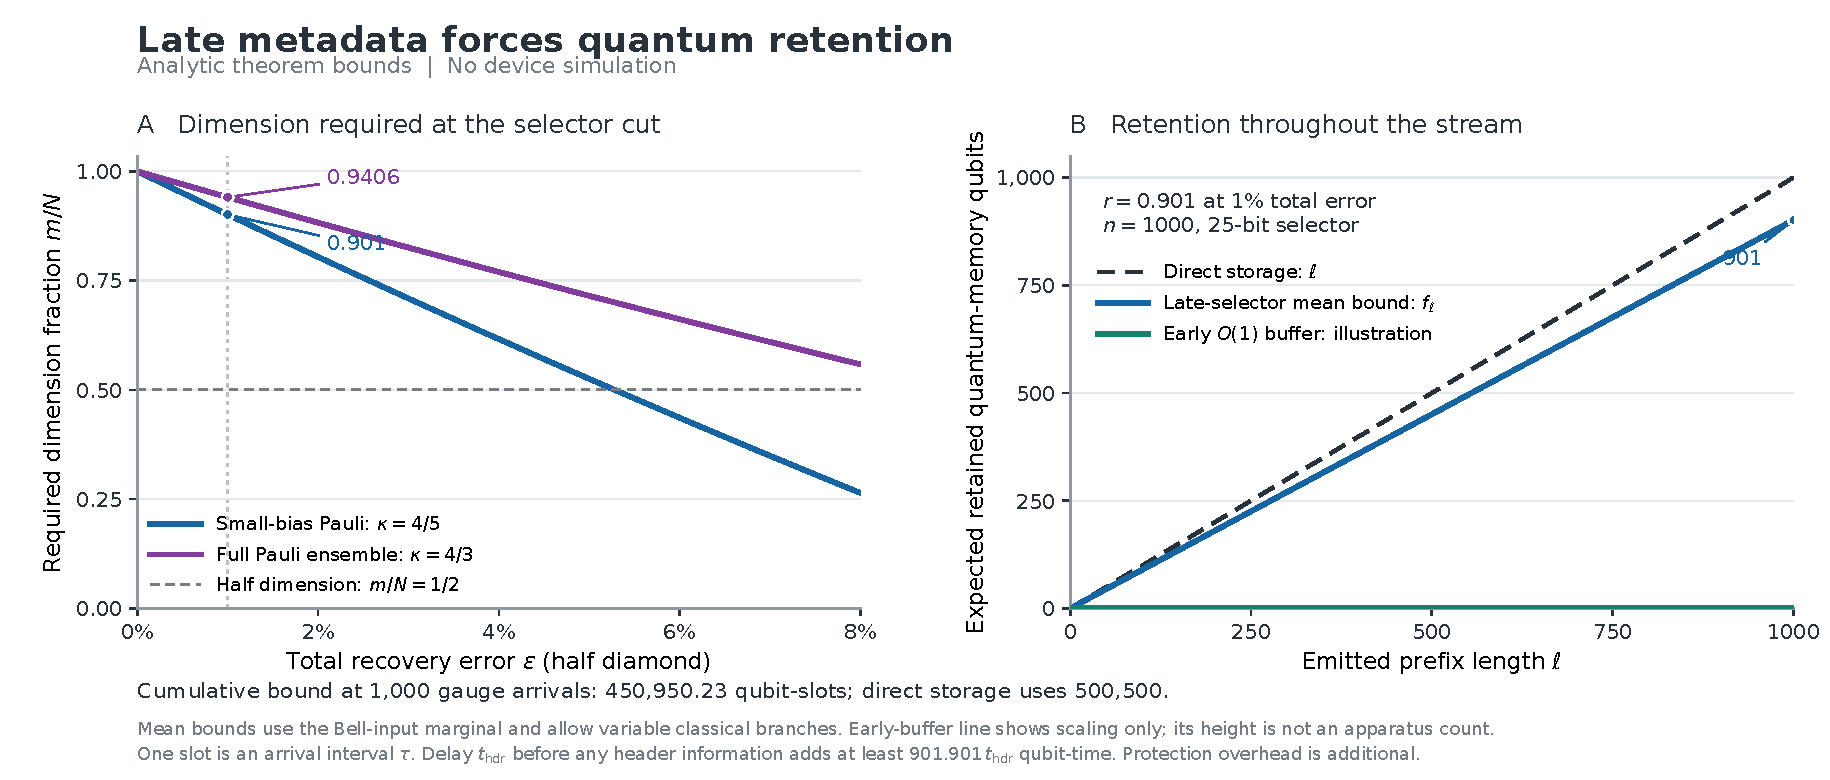
\includegraphics[width=\linewidth]{figures/causal_memory_bounds.pdf}
\caption{Analytic dimension and mean-retention bounds. The early-buffer line
illustrates constant scaling, not an exact apparatus count. With 1000 gauge
carriers and one-percent error, the pre-record expected receiver exposure is
at least $450{,}950.22834\,\tau$ qubit-time. Direct storage uses
$500{,}500\,\tau$ over those intervals. All physical protection is additional.}
\end{figure}

\section{The complete early-record quantum operation}
Write $U_j$ as a product of disjoint local factors. Let $\Pi_z$ refine their
joint spectral projectors, with $U_j\Pi_z=u_z\Pi_z$, $|u_z|=1$. The controlled
encoding obeys the exact instrument identity
\begin{equation}
 (I\otimes\Pi_z)V_j=
 \left[\operatorname{diag}(u_z,1)H\right]\otimes\Pi_z. \label{eq:instrument}
\end{equation}
For an arbitrary initial $\rho_{RQ}\otimes\Gamma_{GF}$, where $F$ can be an
inaccessible gauge purifier, the unnormalised conditional output factors as
\begin{equation}
 (I_R\otimes W_z)\rho_{RQ}(I_R\otimes W_z^\dagger)
 \ \otimes\ \Tr_G[(\Pi_z\otimes I_F)\Gamma_{GF}(\Pi_z\otimes I_F)],
 \quad W_z=\operatorname{diag}(u_z,1)H.
\end{equation}
The outcome probability is independent of the payload and reference. The
receiver measures the local spectral projectors as carriers arrive, stores
their eigenphase product classically, and applies $W_z^\dagger$ to the final
flag. The result is exactly $\rho_{RQ}$ on every branch. The anchor branch
uses $V_0=I$ and no correction.

For a Pauli word this means measuring each carrier in its indicated $X,Y,Z$
basis, discarding identity factors, and retaining only the parity $b$ of
negative eigenvalues. The flag correction is $HZ^b$: first $Z^b$, then $H$.
The receiver uses no inter-carrier quantum gate and no coherent delay for the
gauge. At most one arriving carrier, a fixed meter ancilla and the output flag
need be present. The source record, field arithmetic and timing counter use
$O(\log n)$ classical bits, and the measured outcomes need only one parity bit.

The positive operation works for \emph{any} gauge state independent of the
payload/reference, including correlations between gauge carriers and hidden
purifiers. The hard theorem uses the actual tracial gauge. No bath purifier,
preparation label, source measurement or coherent return link is supplied.
The record gives the \emph{source encoding program}; the eigenvalues used for
correction are measured from the actual emitted particles.

For a CNOT factor, even a two-qubit eigenmeasurement is unnecessary:
\begin{equation}
 \operatorname{CNOT}|c\rangle_Z|b\rangle_X=(-1)^{cb}|c\rangle_Z|b\rangle_X.
\end{equation}
Separate $Z$ and $X$ measurements and a Boolean AND provide its eigenvalue.
Fixed-range matching factors need only a bounded number of pending classical
outcomes, including wraparound pairs.

The strongest simple late-record architecture is to keep every gauge carrier
and the flag. Once the record arrives, it performs these same local
measurements and correction. This post-record readout uses $O(n)$ quantum
operations rather than a large coherent inverse. The lower bound concerns its extensive
retained memory, not an invented computational bottleneck. Known-basis
environment-assisted correction is established \cite{gw}; the new theorem
quantifies what the timing of the basis record costs in this payload task.

\section{Physical source, timing, errors and qualification}\label{sec:bill}

\subsection{An explicit one-flag Pauli source}
The source holds the unknown payload flag and a classical branch/seed record.
In the nonanchor branch it applies $H$ to the flag, then interacts it once with
each incoming carrier $I/2$ through the specified controlled Pauli. Each carrier
leaves permanently after that encounter. Finally, a full SWAP transfers the flag
to a fresh outgoing carrier and leaves the original source maximally mixed.
The original source is discarded. The source needs one coherent payload qubit,
one current carrier and $O(\log n)$ classical program storage.

The same record can be emitted through classical signalling, or through the
same particle stream by swapping physical computational-basis control bits into
fresh tracial carriers. The latter uses $L$ extra carriers. In the early version,
the source keeps a classical copy of the seed for its subsequent gate program;
preparing and retaining that duplicate costs $O(L)$ classical bit writes and
storage. These are explicit source-controller records, not bath purification
keys. Both versions can use the same duplicated classical preparation. Record
slots, source gates, carrier labels and arrival times are fixed and do not leak
the selector before its declared disclosure.

For example, a universal local gate cell with calibrated CNOT, $H,S,X$ and
SWAP operations implements each controlled Pauli with at most five one- or
two-qubit elementary gates, including negative-control conjugation. Source
work is at most $5n+O(L^2+1)$ such gates with a conservative serial metadata
routing layout. The receiver uses at most two basis rotations and one readout
per carrier, a parity update, and two final flag gates. All controls have fixed
local arity and bounded norm. The source encounters here are strong finite
gates; the proof does not claim small per-encounter action.

Peak and slew can both be finite. Write the Hamiltonian as $\hbar g(t)G$
with $\norm G=1$, so $J$ and $S$ below bound $|g|$ and $|\dot g|$.
For area $A$ (at most $\pi/2$ for the involution gates), a pulse with
peak at most $J$ and slope at most $S$ uses a triangular envelope of duration
$2\sqrt{A/S}$ if $A\le J^2/S$, or a trapezoid of duration $A/J+J/S$ otherwise.
Its constant generator makes the area calculation exact. Switching and
settling between available generators is separately charged. If this native
set is unavailable, a supplied local compiler and its cost are required;
bounded norm alone does not create arbitrary gates.

A circuit meter can reuse one ancillary qubit but must prepare/reset it for
each local readout: $O(n)$ meter initializations, with their purity, time,
energy and errors, belong in the receiver bill. A direct physical detector
has corresponding reset and readout costs. Constant retained quantum memory
does not mean constant cumulative preparation resources.

If a caller can instead command an immediate full SWAP of the initial source,
that simpler interface exports the payload directly. Our comparison fixes the
emitter's declared program and varies when its independent classical record
is available. The theorem supplies no reason to build this encoder solely to
transfer a qubit, and no claimed advantage over direct SWAP access. Its purpose
is a sharp receiver-memory boundary for a physically specified mixed stream.

\subsection{Execution bill}
Let $\tau_g$ bound the duration of a compiled local gate, $\tau_m$ a readout,
$\tau_b$ a metadata bit slot, and $f_c$ the classical bit-operation rate. A
serial sufficient schedule has
\begin{equation}
 T=O\!\left(n(\tau_g+\tau_m+\tau_{\rm reset}+\tau_{\rm route}+\tau_{\rm settle})
       +L^2\tau_g+L\tau_b+\frac{nk^2}{f_c}\right). \label{eq:time}
\end{equation}
Delivery flight times and any clock synchronisation are added. At fixed local
hardware rates, quantum processing is linear and total classical work is
near-linear. Precomputing the whole Pauli word removes online field arithmetic
only by paying $O(n)$ program RAM and the same prior computation.

The source flag must remain coherent for the entire run. A fixed logical source
dimension is not a claim of arbitrarily long protection with fixed noisy hardware.
The early receiver's coherent carrier storage is constant in size and $O(n)$
in total qubit-time at fixed gate/readout cadence. Direct late storage has
$n+1$ coherent qubits and $O(n^2)$ qubit-time. Section~\ref{sec:prefix} proves
the matching quadratic lower bound in expected qubit-time under the maximally
mixed/Bell-marginal input, even with variable classical branch sizes. If serial
field generation lengthens slots, both clocks acquire its paid factor.
Loading/routing the late bank is additional; its post-record recovery is linear.

The tracial hard-source factory must produce the stated independent state. For
independent qubits with Bloch lengths $\beta_i$, the inherited sufficient bound is
\begin{equation}
 \nu_{\rm init}\le\tfrac12\sqrt{\prod_i(1+\beta_i^2)-1}.
\end{equation}
Thus uniform $\beta_i=O(\nu/\sqrt n)$ is sufficient for total initialization
error $\nu$. Ideal independent Pauli twirling with erased/inaccessible keys is
one paid preparation option. Approximate twirls of correlated raw inputs need
composable channel bounds. The positive decoder's exact instrument identity
does not itself require a tracial factory, but the quantitative hard-source
memory claim does.

\subsection{Composable errors and what calibration can establish}
A sufficient positive-reader error bound is
\begin{equation}
 \epsilon_{\rm actual}\le\nu_{\rm prep}+\nu_{\rm record}+\nu_{\rm loss}
 +\sum_{\ell=1}^{G}\delta_\ell+\nu_{\rm storage}+\nu_{\rm timing}.
 \label{eq:errors}
\end{equation}
Each term is a composable half-diamond or outcome-error bound for the actual
history/context in which it is used. A simple uniform allocation requires
$\delta_\ell=O(\epsilon/G)=O(\epsilon/n)$. Classical parity readout errors
also accumulate; fixed raw local error is not a constant-error large-$n$
theorem. For Hamiltonian-norm bound $J_E$, timing error contributes at
most $J_E|\Delta t|/\hbar$ per affected pulse. A declared source memory-noise
rate contributes its rate times the full source exposure. Correlated memory
noise needs a bound for the joint process, not an inferred scalar coherence
time. Fault-tolerant control, if used, has additional physical qubits, cycles,
initialization and calibration costs; none is silently supplied.

If the actual flagged complete emission differs from the ideal by half diamond
$\nu$, under the same fixed emission/record schedule, a receiver with actual
error $\epsilon$ recovers the ideal emission with error at most $\epsilon+\nu$.
The capacity bound therefore uses that sum, assumed at most $1/2$. The
five-bit expander version below is particularly demanding.

Expected occupancy additionally depends on branch probabilities. Define
$f_\ell(r)=\max\{0,\ell(r-2^{-\ell})/(1-2^{-\ell})\}$ as in
\eqref{eq:meanmemory}. For the same receiver instrument, branch-to-capacity
assignment and physical cut in both experiments,
\begin{equation}
 \mathbb E_{\rm actual}q_y\ge
 \max\{0,f_\ell(r_{\epsilon+\nu})-\ell\nu\}. \label{eq:noisymean}
\end{equation}
The ideal rank/chord proof bounds the expectation of
$z_y=\min(q_y,\ell)\in[0,\ell]$. Data processing bounds the two prefix record
laws' total variation by $\nu$, changing this bounded expectation by at most
$\ell\nu$; also $q_y\ge z_y$. Integrating \eqref{eq:noisymean} gives the
actual exposure bound. Fixed timing and absence of extra side channels are
essential: final-channel closeness alone does not control earlier metadata
arrival or arbitrary changes in the clock.

Generic qualification of a constant number of stationary local gate types to
$O(\epsilon/n)$ by tomography costs conservatively
$O(n^2\epsilon^{-2}\log(1/\delta))$ trials. This is an upfront cost, not linear
online processing. End-to-end qualification is also possible: for the random
selector distribution the complete early reader is a qubit channel, so trusted
two-qubit Choi tomography uses $O(\zeta^{-2}\log(1/\delta))$ runs for additive
half-diamond tolerance $\zeta$, each costing the full time \eqref{eq:time}.
Measure the 15 nonidentity two-qubit Paulis to accuracy $h$; then
$\norm{J-\widehat J}_1\le\sqrt{15}\,h$ and
$\dd(\Lambda,\id)\le\norm{\widehat J-\Phi_2}_1+\sqrt{15}\,h$.
Trusted Bell preparation, protection of its reference throughout the run,
readout, selector sampling and stationarity are required. This qualifies an
operation that performs well; it does not improve an inaccurate operation.
It certifies the averaged channel, not every seed separately. A worst-seed
claim requires additional structure or a correspondingly larger qualification.

\section{A constant-selector, fixed-register source}
The logarithmic-record construction has useful robustness and one coherent
source qubit, but its classical state grows with $\log n$. For a separate
fixed-register version, import the explicit 16-generator theorem of Anshu
et al.~\cite{depthone}, already accepted in the warm expander companion. It
gives Hermitian disjoint Pauli/CNOT layers on $n=3s$ qubits, ring range at most
four, with absolute gap $\gamma_0=1/(2\cdot10^8)$.

Use the 16 operators $X\otimes U_j$ and anchor $Z\otimes I$, uniformly.
Equation~\eqref{eq:liftgap} gives
\begin{equation}
 \kappa_0=\frac{32\gamma_0}{17}
 =\frac{16}{17\cdot10^8}\simeq9.4117647\times10^{-9}. \label{eq:tinygap}
\end{equation}
There are 17 labels and a five-bit record. At
$\epsilon\le\kappa_0/16\simeq5.88235\times10^{-10}$, the late reader needs
capacity for at least $n$ qubits. This threshold is fixed independently of $n$ but too small
for a one-percent claim. The small-bias gap cannot be assigned to this source.

The full generator list, lift proof and routing schedule are supplied in the
local-expander implementation companion. Hold the first four ring sites and
use a four-site look-ahead window. Emit in the common order
$5,6,\ldots,n,1,2,3,4$, then flag and record. Every nonwrapping pair has
separation at most four; every wrapping partner lies in the retained boundary.
Ten source qubits suffice for boundary, window, current carrier and flag.
Controlled CNOTs are Toffolis with constant local compilation cost. Pad each
slot to the worst-case duration so labels and timing do not disclose $j$.
Small cases use the same finite buffer.

This is a time-programmed finite source with $O(n)$ instructions and an
explicitly paid external clock/horizon, not an immutable time-homogeneous
thermal generator. An internal position counter costs $O(\log n)$ classical
bits if that timing service is removed. The flag and boundary carriers need
protection for $O(n)$ time; a fixed logical register does not make this free.

With early $j$, individual control-$Z$/target-$X$ measurements give every
CNOT eigenvalue. At most four pending classical outcomes plus parity are
needed; no coherent periodic buffer is required. With late $j$, the main
theorem and every-prefix bound apply even to collective compression.
The selector can alternatively be an arbitrary constant-dimensional quantum
input emitted last: retaining the outputs makes the controlled encoding
invertible, and classical-selector subcases prove the lower bound. The early
protocol instead assumes a classical selector and does not preserve its
unknown quantum coherence.
In that variant the five selector qubits also count as coherent source storage,
and their controlled local gates need their own constant-size compilation.

\begin{table}[ht]
\centering\small
\begin{tabular}{@{}p{0.23\linewidth}p{0.22\linewidth}p{0.18\linewidth}p{0.27\linewidth}@{}}
\toprule
Construction & Record bits & Certified $\kappa$ & Paid source storage\\
\midrule
Uniform Pauli & $2n+1$ & $4/3$ & One coherent flag; $O(n)$ classical bits\\
Small-bias Pauli & $2\lceil\log_2(4n-2)\rceil+1$ & $4/5$ & One coherent flag; $O(\log n)$ classical bits\\
Local expander & $5$ & $16/(17\cdot10^8)$ & Ten coherent registers; fixed selector; external time program\\
\bottomrule
\end{tabular}
\caption{Complete but different constructions. Their source, record and gap
resources cannot be interchanged. A current carrier and meter add fixed workspace.}
\end{table}

\section{Comparison with the strongest applicable approaches}
Ballester, Wehner and Winter already show that one Boolean answer after a late
basis choice can require full quantum memory for perfect prediction
\cite[Theorem 6.6]{bww}; their discussion after that construction raises the
near-perfect case. The bare late-choice phenomenon is therefore not new.
Bluhm, Rauber and Wolf already allow unrestricted classical side records and
prove exact measurement-relative incompressibility and fixed-family small-error
stability \cite[Theorem 5.1]{brw}. Their compactness proof does not supply a
dimension-uniform numerical threshold. Their common decompressor preserves
specified observables for all input states.

Ioannou et al.~\cite{simulability} provide the closer operational framework:
one quantum/classical compression followed by setting-dependent measurements,
with a low-rank Kraus characterization. Their analytic robustness bounds for
the full unitarily symmetric family of noisy rank-one projective measurements
are substantive prior results. That all-measurement premise does not follow
from our finite family of balanced binary probes and its average score, so
those bounds do not directly replace the gap-dependent implication here.
Setting-dependent late measurements themselves are not a new model.

The lower bound uses only average discrimination of the finite binary probes;
it does not require preservation of their statistics on every input. Each
selector may choose a different decoder returning only one encoded qubit.
Equation~\eqref{eq:bridge} connects this to one analytic reconstruction, and
the gap yields the explicit dimension bound. The
arbitrary-reference encoding, physical stream, and causal prefix argument
complete the operation and its memory-exposure cost. Petz recovery,
commutator rigidity and Schmidt-number bounds remain existing machinery.

The early protocol is an instance of environment-assisted correction
\cite{gw}. An equally informed early-record receiver can use the same local
measurements; no advantage over that baseline is claimed. Classical small-bias
sets and their Pauli use are prior machinery \cite{aghp,as}, and the five-bit
construction imports the local expander \cite{depthone}. We do not claim better
expanders, encryption, or a first measurement-relative compression theorem.

Pure-input coherent absorbers and collectors use a different physical resource:
actual pure input ports \cite{absorber}. An inaccessible purifier cannot be
substituted for an observed output. Small matrix-product bond dimension alone
does not construct a CPTP compression. The present hard family strengthens a
whole-output obstruction to one arbitrary payload, but is not the homogeneous
weak partial-SWAP channel. Its specialised small-memory receiver remains open.

\section{Executed evidence and reproducibility}\label{sec:evidence}
The package contains complete proofs, programs, machine-readable receipts and
the independent audits. These audits are by separately tasked collaborating
agents, not external peer review or a proof-assistant certificate.
The following are executed finite calculations, not
hardware demonstrations or numerical replacements for the theorem.

\begin{itemize}
\item The actual local-measurement decoder was checked for all Pauli selectors
and anchors for $n=1,2,3,4$: 344 cases. Its full flag-plus-gauge input Choi map
equals partial trace, with maximum normalised-Choi half-trace residual
$3.89\times10^{-16}$. Correlated mixed GHZ gauge checks give residual at most
$9.99\times10^{-16}$.
\item Direct commutator superoperators for the uniform Pauli family at
$n=1,2,3$ have a one-dimensional kernel and gap $4/3$, to numerical precision.
Thirty-two hybrid compression examples, including nonunital amplitude damping,
reset, classical block records and singular baselines, obey $q_j\ge t_j^2$,
$F_e\le m/N$ and the gap bound. Maximum trace-preservation residue is
$3.31\times10^{-15}$. Two examples saturate the latter rank and gap steps.
\item Measuring one gauge qubit in $Z$ before the record, retaining that
classical result, and then applying the specified late decoder gives
$(5/6)\id+(1/6)\Ad_X$ for the uniform Pauli-plus-anchor family.
Checks at $n=1,2,3$ have Choi residual at most $3.92\times10^{-16}$; its
half-diamond error is analytically $1/6$. This is a baseline, not an SDP optimum.
\item Exact finite-field and character checks were run for the small-bias
construction at $n=1,2,3,4,5,8$. For $n=1000$, the field polynomial
$x^{12}+x^3+1$ was found after five candidate tests, and one complete 1000-site
Pauli program was generated. No 1000-qubit density matrix was simulated.
\end{itemize}
The Choi residuals above are not reported as numerically evaluated diamond
norms. The analytic identities establish the reference-uniform statements.
Large source factories, calibration, bounded-noise hardware and protected
memories were not simulated.

\section{Independent completed companions}\label{sec:companions}

\subsection{Restricted partial-SWAP receiver obstruction}
A source collides with fresh $I/2$ qubits at angle $0<\theta<\pi/2$. A single tracial
receiver qubit then uses an arbitrary predetermined partial-SWAP angle on each
outgoing particle and discards it. With $c=\cos\theta$, $s=\sin\theta$, its
depolarizing visibility is uniformly bounded by
\begin{equation}
 |B_N|\le L(\theta),\qquad
 L(\theta)^2=\frac{s^2}{1+c^2}+\frac{32s^4}{(3-c)^2}.
\end{equation}
An arbitrary final decoder has half-diamond error at least
$\tfrac34\max\{0,1-L(\theta)\}$. At $\theta=0.1$ this is $0.6928864$.
The proof uses a closed three-dimensional operator recurrence; 103 direct
$8\times8$ checks have maximum discrepancy $3.34\times10^{-16}$. It excludes
this scalar receiver, not pure or larger memories, general instruments,
measurement feedback, subsystem codes or block compression. No positive
general homogeneous weak-stream receiver was obtained.

\subsection{Finite thermal intervention for hidden linear dynamics}
For a certified observable all-even OU system
$dX=AX\,dt+\sqrt{2D}\,dW$, $Y=CX$, with $A$ Hurwitz and $D>0$, a common
thermal port scaling all diffusion by $1+u(t)$ while preserving $A$ supplies
new information absent from the warm force-only interface. A raised-cosine
pulse $u(t)=\eta\sin^2(\pi t/h)$ has an invertible covariance transfer
\begin{equation}
 \mathcal T_A=\eta\omega^2(e^{h\mathcal L_A}-I)
 [\mathcal L_A(\mathcal L_A^2+\omega^2 I)]^{-1},\quad
 \mathcal L_A(Z)=AZ+ZA^T,\quad\omega=2\pi/h.
\end{equation}
Random hot/control assignment gives a martingale-unbiased difference of
post-pulse covariance matrices on one continuously running specimen, without
hidden resets. Shifted tagged moments recover unknown $A,D$ up to similarity
and the model's native entropy production, with declared order, observability,
anti-aliasing, diffusion-positivity and thermal-reach premises. Inversion uses
a Stein solve and Lyapunov-map applications, $O(d^3)$ classical arithmetic.

The companion pays exposure, moments, conditioning, finite bins, digitisation,
temperature slew, calibration and drift errors. A million no-reset cycles were
executed on a two-dimensional model: inferred entropy rate $21.07725$ versus
$20.25$. Its conservative confidence radius is too loose to certify that
displayed error. General covariance identification is a strong baseline
\cite{kost}; no efficiency superiority or arbitrary hidden-dissipation coverage
is claimed. Thermodynamic entropy interpretation requires the declared physical
state variables, parity and bath model; unseen extra modes remain outside it.

\subsection{Translational force from raw blurred images}
The other independent construction uses a Stokes virtual field and one acquired
radial point-spread second moment. Its quadratic displacement kernel is
separately biharmonic/harmonic, so a finite Laplacian correction cancels the
specified radial blur exactly. Five weighted image covariances and a positive
normalizer give a translational-force current; a reciprocal identity supplies
the force with paid boundary, forcing and finite-lag terms. An explicit annular
translation field and manufactured-flow checks close the mechanical operation.

This requires the stated optical-volume access, independent particle-pair law,
PSF shape/support and moment calibration, geometry, and positive normalization.
The direct estimator can cost $O(h^{-4})$ records as lag $h$ shrinks. The
executed reciprocal force $1.9000352368911049$ agrees with direct wall stress
$1.9000352368911066$; these are deterministic quadrature, not measured images.
Pizzetti/Faxen corrections, reciprocal-force formulas and correlation-based
stress inference are strong prior machinery. An equally informed implementation
can compile the same weighted covariances. No general advantage over a direct
force balance or the best image-correlation estimator is established.

\section{Preserved knowledge and unresolved boundaries}
The warm results are retained unchanged, with governing sources and access
contracts. They are premises, not subjects of another validation campaign.

\begin{enumerate}
\item \textbf{Fourth-order action law.} Fresh finite tracial ancillas are
independent of source/reference and retained systems conditional on genuine
classical history. No coherent return or extra source measurement/reset is
supplied. With whole-encounter actions $a_j$,
$b=\prod_j[1-\min(1,4a_j^4)]$, $\alpha=1-b$ and $c=1-d^{-2}$,
every decoder has error at least $c(1-\sqrt\alpha)\ge cb/2$, with the accepted
acquired-information bound. Classical feedback and finite stopping are included
under that contract. Pathwise charge
$\sum_j-\log[1-q(a_{j,h})]\le C_*$ gives $b=e^{-C_*}$; this is not an
expected-action or free-postselection result.
\item \textbf{Exact partial-SWAP channels.} The acquired channel is
$\mathcal C_N(\rho)=\Tr_S U(\rho\otimes I_B/d^N)U^\dagger$.
Reversing the circuit on all outputs and an independent tracial dummy gives
$\mathcal D_N\mathcal C_N=(1-r)\id+r\mathcal R_{I/d}$, with
$r=\prod_j(1-\sin^4\theta_j)$. Original source and purifiers are absent.
The explicit half-diamond error is $cr$ and every decoder has error at least
$c(1-\sqrt{1-r})$, the factor-two guarantee. This is an exact channel identity,
not exact finite-weak-collision recovery.
\item \textbf{Independent modules.} Product emission allows arbitrary
entangled inputs/references and collective final decoding. For
$V=\prod_i(1-c_i r_i)$, the explicit reader has error $1-V$ and every
collective decoder error at least $1-\sqrt V$, with the sharper accepted
finite-dimension version available. Active coupling that destroys product
emission is outside the theorem.
\item \textbf{Forgetting and acquisition.} Source visibility
$\prod_j\cos^2\theta_j$ decays on the quadratic collision scale while
output recovery uses the quartic scale. Identical reduced source dynamics can
have different physical acquired channels. Factory, routing, calibration,
protection, peak and slew costs remain part of those results.
\item \textbf{Earlier families.} Unknown-support rare-failure acquisition,
the fixed-start lifetime bound, correlated product-invariant computation,
finite collision/factory implementation and separate equilibrium-safe
initialization retain their operating refresh backbone, declared local port
reach, starting-mass and precision costs. The all-strength hidden-dephasing
obstruction, finite effusion protocol, protected readout and pure-Weyl-port
recovery retain their supplied physical resources.
\item \textbf{Both prior nonquantum companions.} The force-port OU
nonidentifiability construction and directed-local-dynamics prediction
obstacle remain at their original scopes. The latter uses an ideal local
compiler and is not a fault-tolerant physical complexity separation. The new
thermal pulse adds a different physical port and does not invalidate the
earlier identical-transcript obstruction.
\item \textbf{Pure-port weak export.} The earlier effort to remove the
strong-export threshold did not produce an efficient finite decoder.
Forgetting and abstract recovery existence did not close overlapping output
recovery and boundary correlations. This remains a construction gap, not a
negative theorem. The completed pure coherent Weyl collector remains an
available stronger-export baseline with growing control/precision and paid
protected memory.
\end{enumerate}

The homogeneous weak partial-SWAP stream's small-memory, near-linear causal
receiver also remains unresolved. The present result changes the general
question: there is no universal small-memory inference from payload dimension
alone, and in the programmed-source class from source-register dimension alone.
A short early control record supplies an exact constant-workspace reader in
the constructed family. The same record delivered late costs extensive memory
and quadratic retained quantum exposure. These conclusions and their stated
limits are the completed scientific consequence of this return.

\begin{thebibliography}{99}\footnotesize
\bibitem{bww} M. A. Ballester, S. Wehner and A. Winter.
State Discrimination With Post-Measurement Information.
\emph{IEEE Trans. Inf. Theory} 54, 4183--4198 (2008).
\url{https://arxiv.org/abs/quant-ph/0608014}.
\bibitem{brw} A. Bluhm, L. Rauber and M. M. Wolf.
Quantum Compression Relative to a Set of Measurements.
\emph{Ann. Henri Poincare} 19, 1891--1937 (2018).
\url{https://arxiv.org/abs/1708.04898}.
\bibitem{gw} M. Gregoratti and R. F. Werner. Quantum Lost and Found.
\emph{J. Mod. Optics} 50, 915--933 (2003).
\url{https://arxiv.org/abs/quant-ph/0209025}.
\bibitem{simulability} M. Ioannou, P. Sekatski, S. Designolle,
B. D. M. Jones, R. Uola and N. Brunner.
Simulability of High-Dimensional Quantum Measurements.
\emph{Phys. Rev. Lett.} 129, 190401 (2022).
\url{https://arxiv.org/abs/2202.12980}.
\bibitem{aghp} N. Alon, O. Goldreich, J. Hastad and R. Peralta.
Simple Constructions of Almost $k$-wise Independent Random Variables.
\emph{Random Structures \& Algorithms} 3, 289--304 (1992).
\url{https://doi.org/10.1002/rsa.3240030308}.
\bibitem{as} A. Ambainis and A. Smith.
Small Pseudo-Random Families of Matrices: Derandomizing Approximate Quantum
Encryption. RANDOM 2004.
\url{https://arxiv.org/abs/quant-ph/0404075}.
\bibitem{depthone} A. Anshu, S. Balasubramanian, J. Haferkamp, A. W. Harrow
and X. Tan. Depth-1 expanders on the unitary group and applications.
Preprint arXiv:2609.01605v1, Theorem 2.2 (2026).
\url{https://arxiv.org/html/2609.01605v1}.
\bibitem{absorber} F. Girotti, A. Godley and M. Guta.
Estimating quantum Markov chains using coherent absorber post-processing
and pattern counting estimator. \emph{Quantum} 9, 1835 (2025).
\url{https://arxiv.org/abs/2408.00626}.
\bibitem{kost} O. Kost et al. Unobservable Systems: No Problem for Noise
Identification. Preprint arXiv:2505.23983; comparison uses v2.
\url{https://arxiv.org/html/2505.23983v2}.
\bibitem{astra} Accepted Astra construction packages at fixed revision:\\
{\small\texttt{324acb589443002bf8d529cc15e160129c5e36d2}}.
\url{https://github.com/harjassand/astra-research-knowledge/tree/324acb589443002bf8d529cc15e160129c5e36d2/research/returns}.
The supplied warm mixed-collision acquisition package and its unchanged
proofs, execution records and two companions are preserved separately and
indexed in this return's \texttt{README.txt}.
\end{thebibliography}
\end{document}
